After the detector simulation described in \Sec{sec:eventgeneration}, the simulated data has the exact same format as the real collision data recorded at the CMS experiment. Therefore the same software can be used for the reconstruction of both simulation and real data. In \Sec{sec:reco}, the object reconstruction for physics analysis is shown. After reconstructing the objects, the objects are connected to physics objects need to be identified. This identification is explained in \Sec{sec:id}. A basic event selection is made for selecting signal like events. The necessary event requirement are discussed in \Sec{sec:selection}. 

The analysis uses signal and background regions to constrain the huge \SM\ background compared to the expected signal. \Sec{sec:regions} discusses each region that is entering the analysis. On top of the use of background estimation from control regions, backgrounds that have  prompt leptons  contaminated by real leptons either
from decays of tau leptons or from hadronized mesons or baryons
(collectively commonly referred as ``non-prompt leptons") as well as by
hadrons or jets misidentified as leptons\footnote{These two classes
of contamination will be referred to as not prompt-lepton (\NPL) samples.} are
evaluated with a data-driven method discussed in \Sec{sec:NPL}.

\section{Object Reconstruction}
\label{sec:reco}
In \fig{fig:transversecms}, the particle interaction in a transverse slice of the CMS detector is shown. The particles enter first the tracker where charged particle trajectories, so-called tracks, and origins or vertices are reconstructed from signals (hits) in the sensitive layers. Charged particles get bent by the magnetic field making it able to measure the electric charges and momenta of charged particles. In the ECAL, the electron and photons are absorbed and the corresponding electromagnetic showers are detected as clusters of energy in adjacent  cells.From this, the energy and the direction of the particles can be determined. The charged and neutral hadrons can initiate a hadronic shower in the ECAL that is fully absorbed in the HCAL. The clusters from these showers are also used to estimate the energy and direction. Muons and neutrino's pass through the calorimeters without little to no energy loss. The neutrino's escape the CMS detector undetected while muons produce hits in the muon detectors. 
\begin{figure}
	\centering
	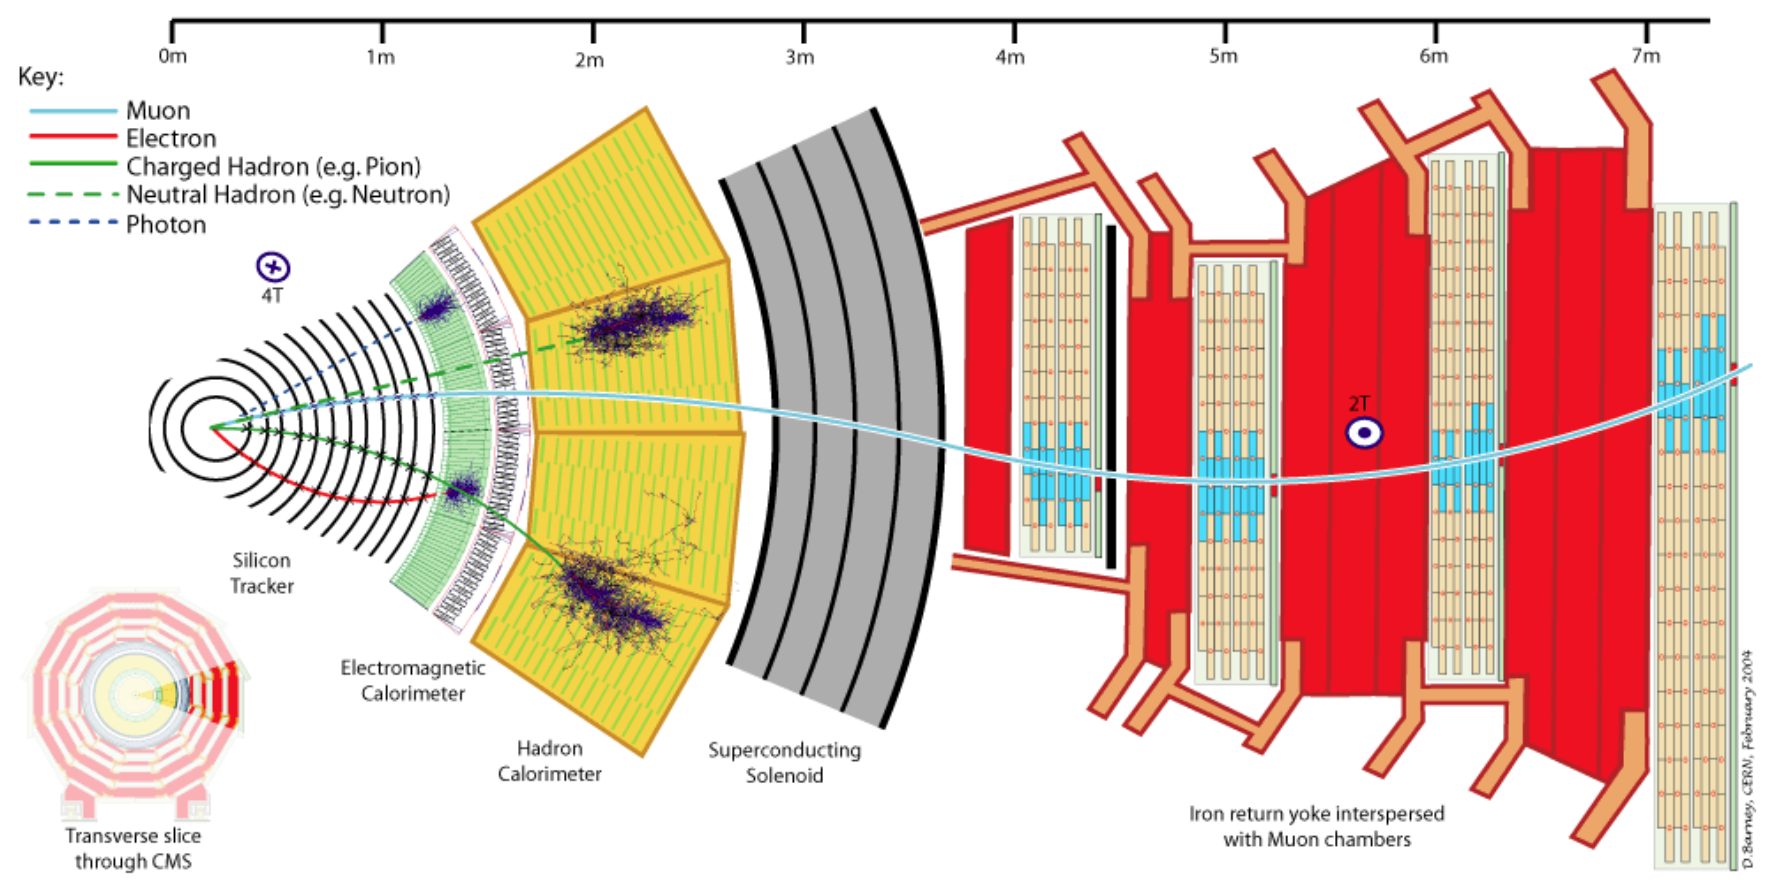
\includegraphics[width=1.\linewidth]{4_EventRecoSelect/Figures/transversecms}
	\caption{Cross-section of the CMS detector with all parts of the detector labelled. This sketch shows the specific particle interactions from a beam interaction reign to the muon detector. The muon and charged pion are positively charged, the electron is negatively charged. Figure taken from~\cite{CMS-PRF-14-001}. }
	\label{fig:transversecms}
\end{figure}

The traditional hadron colliders reconstruction is as follows. The reconstruction of isolated photons and electrons is primarily done by the ECAL, while the identification of muons is based on the muon detectors. Hadrons and photons form jets which are measured by the calorimeters without any contribution from the tracker or muon detectors. Jets can be tagged using the tracker as coming from hadronic \Ptau\ decays or \Pbottom\ hadronisation based on the properties of the properties the relevant charged particle tracks. The missing transverse energy is defined as the vectorial sum of the undetectable particle transverse momenta, and can be reconstructed without any information from the tracker. 
The particle flow (PF)~\cite{CMS-PRF-14-001} reconstruction correlates the tracks and clusters from all detector layers with the identification of each final state particle, and combining the corresponding measurements to reconstruct the properties. Here, the muon is identified by a track in the inner tracker connected to a track in the muon detector as described in \Sec{sec:MuonTrack}. The electrons are identified by a track and ECAL cluster, and not connected to an HCAL cluster as described in \Sec{sec:ElectronTrack}. The ECAL and HCAL clusters without a track link identify the photons and neutral hadrons, while the addition of the tracker determines the energy and direction of a charged hadron. 


Coarse-grained detectors can cause signals of different particles to merge and reduce the ability of identifying and reconstructing the particles. Therefore, particle flow identification requires sufficiently segmented subdetectors such that a global event description is possible. From a list of identified particles that are reconstructed from a combined fit of all relevant measurements, the physics objects are determined. The CMS detector is built to meet to requirements of the particle flow reconstruction. It has an efficient and pure muon identification system, a hermetic HCAL with coarse segmentation, a higher segmented ECAL, a fine-grained tracker and a large magnetic field to separate the calorimeter deposits of charged and neutral particles in jets. 

%http://slideplayer.com/slide/2779564/
%http://slideplayer.com/slide/4496166/
\subsection{Charged particle tracks}
An iterative tracking algorithm is responsible for the reconstruction of the tracks made by charged particles in the inner tracking system. Each iteration consists of four steps~\cite{Bayatian:922757}: the track-seed generation, the pattern recognition algorithm, removal of track-hit ambiguities and a final track fit. 

The seed generation is the first step. It consists of finding reconstructed hits that are usable for seeding the subsequent track-finding algorithm. They are identified from a group of at least three reconstructed hits in the tracker, or from a pair of hits while requiring the origin of the track segment to be compatible with the nominal beam-collision point. Since the pixel has a higher granularity compared to the strip tracker, its seed generation efficiency is higher. The overall efficiency exceeds 99\%.
The second step of each iteration, the pattern recognition algorithm, uses the seeds as a starting point for a Kalman filter method~\cite{FRUHWIRTH1987444,Billoir:1989mh}. This algorithm extrapolates the seed trajectory towards the next tracker layer taking into account the magnetic field and multiple scattering effects. The track parameters are updated when a compatible hit in the next layer is found. This procedure continues until the outermost layer is reached.
Since the Kalman filter method can result in multiple tracks associated to the same seed, or different tracks sharing the same hits, a removal of ambiguities is necessary. This ambiguity resolving is done by removing tracks that are sharing too many hits from the list of track candidates. The tracks with the highest number of hits or with the lowest $\chi^2$ in the track fit is kept. 
The updated track parameters are then refitted using the Kalman filter method, where all hits found in the pattern recognition step are taken into account. The fit is done twice - once outwards from the beam line towards the calorimeters, and inwards from the outermost track hit to the beam line -, improving the estimation of the track parameters. 

All hits that are unambiguously associated to the final track are removed from the list of available hits. In order to associate the remaining hits, the procedure is repeated with looser track reconstruction criteria. The use of the iterative track reconstruction procedure has a high track finding efficiency, where the fake track reconstruction rate is negligible. 
For muons, this results in a global track reconstruction efficiency exceeding 98\%, and 75-98\% for charged hadrons. 

\subsection{Following the Muon's Footsteps}
\label{sec:MuonTrack}
% see http://www.bo.infn.it/sminiato/sm16/03_Mercoledi/Mattina/01_Battilana.pdf
% see https://arxiv.org/pdf/1510.05424.pdf
% see https://twiki.cern.ch/twiki/bin/view/CMSPublic/MuonDPGPublic160729
The muon reconstruction~\cite{Chatrchyan:2012xi} has three subdivisions: local reconstruction, regional reconstruction and global reconstruction. The local reconstruction is performed on individual detector elements such as strip and pixel hits in the inner tracking system, and muon hits and/or segments in the muon chambers. Independent tracks are reconstructed in the inner tracker - called tracker tracks -  and in the muon system, called standalone muon tracks.
Based on these tracks, two reconstructions are considered.

The outside-in approach is referred to as Global Muon reconstruction. 
For each standalone muon track, a inner tracker track is found by comparing the parameters of the two tracks propagated onto a common surface. Combining the hits from the tracker track and the standalone track, gives a fit via the Kalman filter technique~\cite{FRUHWIRTH1987444,Billoir:1989mh} for a global muon track. 

The second approach is an inside-out reconstruction, creating tracker muons. 
All candidate tracker tracks with a \pt$>0.5$ \GeV\ and total momentum p$>2.5$ \GeV\ are extrapolated to the muon system taking into account the magnetic field, the average expected energy losses, and multiple Coulomb scattering in the detector material. The extrapolated track and the muon segments are considered matched when the difference in the position in the x coordinates is smaller than 3~\cm, or when the ratio of this distance to its uncertainty is smaller than four. When at least one muon segment - DT or CSC hits -  matches the extrapolated track, the corresponding tracker track is indicated as a tracker muon. 

For low transverse momenta ($\pt \lesssim$ 5~\GeV), the tracker muon reconstruction is  more efficient than the global muon approach. This is due to the fact that tracker muons only require a single muon  segment in muon system, while the global muon approach requires typically segments in at least two muon stations. These tracker muons are used for identifying muons from the hadronisation of \Pbottom or \Pcharm  quarks. The global muon approach typically improves the tracker reconstruction for $\pt\gtrsim$ 200~\GeV. These are labelled isolated when in a cone of $\Delta R = \sqrt{\Delta\phi^2 + \Delta \eta^2} = 0.3$ around the muon, the sum of the transverse momenta of additional tracker tracks and energy deposits in the calorimeter is less than 10\% of the muon's transverse momentum.
\subsection{The path of the Electron}
\label{sec:ElectronTrack}
% see also https://arxiv.org/pdf/physics/0512097.pdf
% https://cds.cern.ch/record/1563583/files/ATL-PHYS-PROC-2013-206.pdf
% http://cds.cern.ch/record/1704291
The electrons in CMS radiate more than 70\% of their energy in the inner track through bremsstrahlung before reaching the ECAL. This has as consequence that the electron tracks are increasingly curved in the magnetic field as a function of its flight distance. Standard tracking algorithms are based on Kalman filtering which assume that the energy loss is Gaussian distributed, and are therefore not suitable to fit the electron tracks. A different filtering algorithm, the Gaussian sum filter (GSF) \todocite is used in the electron track reconstruction instead. 

In CMS, the electrons are reconstructed in two ways. The older ECAL based tracking is developed to identify high energy, isolated electrons. This tracking algorithm starts from ECAL clusters with a transverse energy above 4~\GeV\ and extrapolates from these cluster the position of the hits in the tracker. In order to account for bremsstrahlung, neighbouring clusters in $\eta$ and $\phi$
are grouped together into a supercluster from which then the direction is determined to find the position of the particles in the tracker. This has as consequence that for electrons or positrons in jets, energy deposits of surrounding particles will be entering the supercluster leading to a wrong position of the electron/positron in the tracker. Another disadvantage of the ECAL based tracking is that for low \pt\ electrons, the trajectories will be very curved and the supercluster will not contain all of the energy deposit, leading to a higher misconstruction rate. 

The faults of the ECAL based tracking are lifted by adding a tracker based algorithm. This algorithm uses all the tracks with a \pt higher than 2~\GeV found with iterative tracking as seeds. Iterative tracking uses the Kalman Filter algorithm several times with an average track reconstruction efficiency but high purity. In contrary with a global combinatorial fit, the iterative tracking accepts tracks with a small transverse momentum that are not leaving any energy in the ECAL, and tracks from particles that only interact with the inner tracker layers. When the electron or positron radiated a small amount of energy, the corresponding track can be reconstructed across the whole tracker and safely propagated to the ECAL surface. When there is a larger amount of enrgy radiated however, the pattern recognition might fail  to accommodate for the change in the electron momentum leading to a track reconstructed with a small number of hits. The solution for this is a preselection based on the $\chi^2$ and number of hits and the selected tracks are fitted again with Gaussian-Sum-Filter which can accommodate substantial enery losses across the trajectory. 

The electron seeds from the ECAL- and tracker-based procedures are merged into a unique collection and are then refitted  by using the summed Gaussian distributions as uncertainty per hit in the track fit. 

The electron efficiency is measured in 8~\TeV\ proton collision data to be better than 93\% for electrons with an ECAL supercluster energy of $E_{\mathrm{T}}>20$~\GeV \todocite. For electrons with an  $E_{\mathrm{T}}>25$~\GeV\  in 13~\TeV\ proton collision data, the effiency is about 96\% \todocite.

%Due to the lack of coverage of the two pixel discs in high \abspsrap range, the efficiency drops. 
%The resolution on the transverse momentum for a 100 \si{ \GeV} charged particle is about 2.0\% (FIX ME). 
% see https://twiki.cern.ch/twiki/bin/view/CMSPublic/TrackingPOGPlots2016
\subsection{Primary Vertex Reconstruction}
\todo{Check text with PFlow paper!}
The primary vertex reconstruction should be able to measure the location of all proton interaction vertices in each event: the signal vertex an all vertices from pile up events. 
It consists of a vertex finding and a vertex fitting algorithm and happens in three steps. Tracks are selected  to be consistent with being produced promptly in the primary interaction by imposing requirements on the track parameters~\cite{Chatrchyan:1704291}. By grouping reconstructed tracks according to the $z$ coordinate of their closest approach to the beam line, vertices for all interaction in the same beam crossing are found, at CMS this is done by a deterministic annealing algorithm~\cite{726788} . On top of this, a vertex fitting algorithm like the Adaptive Vertex fitter~\cite{Waltenberger:1166320}, is performed. This creates the three-dimensional primary-vertex position. With this fit, the contribution from long-lived hadron decays is reduced by down weighting the tracks with a larger distance to the vertex. The primary vertex corresponding to the highest sum of squared track transverse momenta is noted as the point of the main interaction. The resolution on the primary vertex is about 14 \si{ \micro \meter} in $r\phi$ and about 19 \si{ \micro \meter} in the $z$ direction for primary vertices with the sum of the track $p_T > 100$ \si{ \GeV} for 2016 data taking.
% numbers from https://twiki.cern.ch/twiki/bin/view/CMSPublic/TrackingPOGPlotsICHEP2016

\subsection{Calorimeter clusters}
The cluster algorithm in the calorimeter 
\begin{enumerate}
	\item detects and measures the energy and direction of stable neutral particles such as photons and neutral hadron, 
	\item separates neutral particles from charged hadron energy deposits, 
	/item reconstructs and identifies electrons and their bremsstrahlung photons, 
	\item contributes to the energy measurements of charged hadrons that don't have accurate tracks parameters, e.g. for low quality and high transverse momentum tracks. 
\end{enumerate}
The clustering is performed separately in each subdetetector: ECAL barrel and endcaps, HCAL barrel and end caps, and the two preshower layers. The HF has no clustering algorithm since the electromagnetic or hadronic components give rise to an HF EM or HF HAD cluster. 

The clustering algorithm consist of different steps. First seeds are identified when cells have an energy larger than the seeding threshold and lager than their neighbouring cells. Then topological clusters are made by accumulating cells that share at least a corner with a cell already in the cluster and an energy above a cell threshold set to twice the noise level. The third step is a expectation maximization algorithm that reconstructs the cluster~\cite{CMS-PRF-14-001}. This algorithm assumes that  the energy deposits are Gaussian distributed  and is an iterative algorithm with two steps at each iteration. A first step calculated the expected fraction if the energy in a certain step, while the second step performs a maximum likelihood fit. The positions and energies of the Gaussian functions are then taken as cluster parameters. 

The calorimeter clusters are used for reconstructing photons and neutral hadrons. The  clusters that are not in the vicinity of the extrapolated charged tracks are easily identified as neutral hadrons or photons. For the energy deposits that overlap with charged hadrons however, the neutral particle energy deposit can only be detected as an excess over the charged particle deposit. For this reason, a good calibration of the electromagnetic and hadronic calorimeter is  vital. 

The ECAL calibration is performed before the hadron cluster calibration or particle identification\footnote{Specifically electron and photon energy corrections are performed after the identification step.}. For Run 1, the ECAL response to electrons and photons as well as the cell-to-cell relative calibration is determined with test beam data, radio active sources, and cosmic ray measurements. For Run 2, the collision data collected at 7 and 8~\TeV\ was used to refine the calibration. The effect of the thresholds in the clustering algorithm are estimated from simulated single photons with energies varying from 0.25 to 100~\GeV. The photons used for the calibration should not have a conversion prior to their entrance to ensure the calibration of single clusters. In all ECAL regions and for all energies, the calibrated photon energies agree with the true photon energies within 1\%.

In contrary to the photons, the hadrons deposit in general energy in both ECAL and HCAL. Since the calorimeter responce in the HCAL depends on the fraction of shower energy deposited in the ECAL, the ECAL and HCAl cluster energyes are recalibrated together to get an estimate of the true hadron energy. Since now the calibration is done for hadrons, single neutral hadrons such as $K_{\mathrm{L}}^0$ are used for determining the calibration constants. The hadrons interactiong with the tracker material are rejected for the calibration purposes. This calibration is checked with isolated charged hadron selected from early data recorded at $\sqrt{s}=0.9, 2.2$ and 7 \TeV.  

\section{Putting the pieces together}
\label{sec:id}
A link algorithm connects the several PF elements from the various CMS subdetectors. It tests any pair of elements in an event and is restricted to considering nearest neighbours in the $\eta\phi$-plane. The quality of the link is determined via the distance between the two elements and PF blocks of elements are formed from elements with a direct link or indirect link through common elements. 


The link between a central tracker track and a calorimeter clusters is made by extrapolating the tracker track to the two layers of the preshower, the ECAL, and the HCAL. If this extrapolated position is within the cluster area, the two are linked. When there are several ECAL or HCAL clusters for the same track, the link with the smallest distance is kept. A dedicated cluster algorithm accounts for the energy of the photons emitted through bremsstrahlung ar for photons that have converted to an electron-positron pair. \\The ECAL to HCAL cluster and ECAL to preshower cluster links are established when the cluster position in the more granular calorimeter, ECAL or preshower, is in accordance with the cluster envelope of the less granular calorimeter (HCAL or ECAL).  When there are multiple HCAL clusters linked to the same ECAL cluster, the link with the smallest distance is kept. This is also true for multiple ECAL clusters with the same preshower clusters. The ECAL supercluster is linked with the ECAL cluster when they share at least one ECAL cell. \\
Nuclear interactions in the tracker can lead to kinks in hadron trajectories as well as the production of secondary particles. This leads to charged particle tracks linked together via a common displaced vertex. The displaced vertices considered should have at least three tracks, with at most one incoming track, and the invariant mass of the outgoing tracks should exceed 0.2~\GeV. \\
The link between a track and the muon detectors is done via local, regional, and global reconstruction as explained in \Sec{sec:MuonTrack}. 


\section{Particle flow identification}
In each PF block the identification and reconstruction follows a particular order where after each identification and reconstruction the corresponding PF elements (tracks and clusters) are removed from the PF block The muons are the first to be identified and reconstructed. These are reconstructed if their momenta are compatible with corresponding track only momenta. Then the electron and its corresponding brehmstrahung photons, are identified and reconstructed by using of the GSF tracking. At the same time, the energetic and isolated photons are identified as well. The remaining element in the PF block are subjected to a cross identification of charged hadrons, neutral hadrons, and photons that arise from parton fragmentation, hadronisation, and decays in jets. The charged hadron candidate is made from the remaining candidates that have a charged particle track associated with them. Then the charged particle energy fraction is subtracted from the calibrated energy of the linked calorimeter clusters and the remaining energy is assigned to the neutral energy. Depending on the excess of neutral energy in the ECAL and HCAL clusters, a photon or a neutral hadron is assigned respectively. The pseudorapidity range of the inner tracker limits the information on the particles charge to $|\eta| < 2.4$. Outside this range a simplified identification is done for hadronic and electromagnetic candidates only. 

\subsection{Muons}
\label{sec:Muon}
A set of selection requirements based on the global and tracker muon properties is responsible for muon identification. The muons are considered isolated when the additional inner tracks and calorimeter energy deposits within a distance to the muon direction in the $\eta\phi$-plane is smaller than 0.3. The muons coming from charged hadron decays or heavy flavour decays need more stringent criteria. This due to the fact that charged hadrons can be misidentified as muons because of e.g. punch-through, or muons can be seen as charged hadrons, and will absorb the erngy deposits of nearby particles. 
\subsection{Electrons and isolated photons}
\label{sec:Electron}
The electrons and photons are reconstructed together as discussed before. An electron candidate seeded from a GFS track is considered an electron when the linked ECAL cluster is not linked to three or more additional tracks. The photon seeds are ECAL superclusters with transverse energies above 10\GeV\ that have no links with a GSF track. After associating photons from brehmstrahung with the associated electrons, the remaining energy is associated to the photons and the photon direction is taken to be that of the supercluster. The electron direction is chosen to be that of the GSF track and its energy is a combination of the ECAL energy with the momentum of the GSF track. Photons are retained if they are isolated, while electrons should satfisy additional criteria based on a multivariate analysis for isolated and non-isolated electrons. 
\subsection{Hadrons (jets) and non-isolated photons}
\label{sec:Hadron}
\subsection{Jets from b-quarks}
\label{sec:bJets}
\subsection{Post processing}
\label{sec:Postprocess}
\subsection{Missing transverse energy}

\subsection{Luminosity}

\subsection{Summary of corrections}

\begin{comment}
% Jet energy scale and resolution in the CMS experiment in pp collisions at 8 TeV
% http://iopscience.iop.org/article/10.1088/1748-0221/12/02/P02014/meta
% atlas http://inspirehep.net/record/1519834

% photobn http://iopscience.iop.org/article/10.1088/1748-0221/10/08/P08010/pdf
\subsection{The particle flow event reconstruction method}
% https://cds.cern.ch/record/2237475?ln=en
% atlas http://inspirehep.net/record/1520722
\subsection{Identification of particles}
\subsubsection{Muon reco and ID}
% trigger and good explenation of ID https://arxiv.org/pdf/1206.4071.pdf
% https://cds.cern.ch/record/2257968/files/DP2017_007.pdf
\subsubsection{Electron reco and ID}
% https://cds.cern.ch/record/2255497/files/DP2017_004.pdf
% https://cds.cern.ch/record/2255497?ln=en
\subsubsection{Jet reco and ID of b quarks}
% jet algorithms 
% http://cms.cern.ch/iCMS/analysisadmin/cadi?ancode=JME-16-003

% Identification of b and c jets in the CMS experiment at the LHC Run 2
% http://cms.cern.ch/iCMS/analysisadmin/cadilines?line=BTV-16-002
% SF https://twiki.cern.ch/twiki/bin/view/CMS/BtagRecommendation80XReReco
%Identification of b quark jets at the CMS Experiment in the LHC Run 2
% https://cds.cern.ch/record/2138504?ln=en

%Identification of c-quark jets at the CMS experiment
%https://cds.cern.ch/record/2205149?ln=en

\subsubsection{Missing transverse energy reconstruction}
\subsection{Calibrations and corrections}
%CMS has been taking collision data since the 13TeV startup of the LHC on 3 June. During this period, the CMS magnet has been kept off due to an issue with the cooling system, so the beams have been used to calibrate and time-in the electronics of the various parts of the detector. These operations, which are largely independent of the magnetic field, are now complete. Meanwhile, the data collected with zero magnetic field can be used for fundamental research, like the measurement of the multiplicity of charged particles produced at the new collision energy of 13 TeV. The issue with the magnet cooling system was identified in the final preparatory phase leading to collisions in the LHC. While preparing for beam in CMS, a problem was found in the system that feeds liquid helium to the CMS superconducting magnet. The problem was diagnosed to be due to oil, which is used in the initial compression stages, reaching the so-called 'cold-box’ of the cryogenic system. The cold-box is a complex system with several sets of filters protecting three turbines along the path of the helium towards the magnet. In order to clean the oil contamination essentially all components of the cold-box have been extracted and replaced. Analysis confirms that there is no oil contamination in the CMS magnet itself or risk to its operation during 2015. The cold-box of is now being stabilised after the cleaning intervention and is being brought back to operational conditions. CMS is confident that, following the LHC technical stop and the beam conditioning run that will start at the end of this week, after the low-intensity and commissioning period, the full magnetic field will be available for the 13 TeV LHC run.
\end{comment}






\section{Event selection}
\label{sec:selection}
\section{Regions and channels}
\label{sec:regions}
\section{Data driven background simulation}
\label{sec:NPL}